\documentclass[../../../../dd.tex]{subfiles}

\begin{document}

	\section{Overview}
		MyTaxiService system architecture has been designed as a 3-tier architecture (Data Tier, Logic Tier and Presentation Tier) to facilitate the development of the system using the MVC software design pattern. In fact the three tiers represent in some way the Model (Data Tier), the Controller (Logic Tier) and the View (Presentation Tier) of the software.
		\\
		The architecture of the system is described by the following figure:
		\begin{figure}[H]
			\centering
			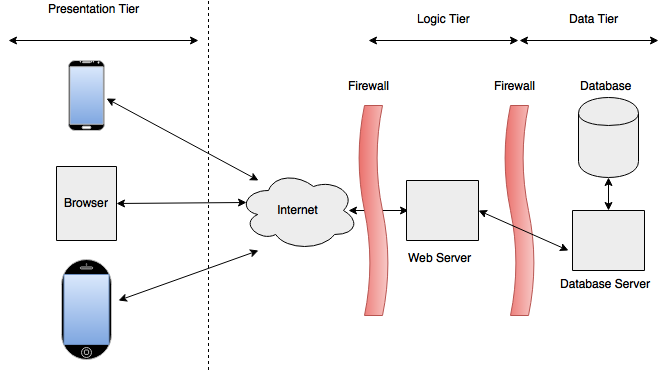
\includegraphics[width=\textwidth, scale=0.5]{../../rasd/IMG/ServerArchitecture.png}
			\caption{System Architecture}\label{fig:SystemArchitecture}
		\end{figure}
		The components of the system are divided in the three tiers:
		\begin{itemize}
			\item In the Presentation Tier there are implemented classes and the objects that compose the view part (what the user see). From this tier users can performing actions to query the system and use the web and mobile applications.
			\item The Logic Tier is the place where are implemented classes and objects that compose the controller (actual logic of the system). This part is in charge of taking requests by the users applications and perform changes on the data. This part is also in charge to notify the applications (presentation tier) of the data changes.
			\item The Data Tier is the place where are implemented the classes and the objects that interact directly with the database. These objects represent the entities of the database and are able to perform creation, modification and deletion of database records.
		\end{itemize}

\end{document}